\chapter{数据表示、位级运算与浮点数}\label{CO02}

\section{进位计数制与位串解释}\label{CO02-radix}

位串的真值由位宽、编码和小数点位置共同确定。1 B=8 bit，B 表示字节，b 表示位。

\[ (a_k\cdots a_0.a_{-1}\cdots)_r=\sum_i a_i r^i,\qquad 0\le a_i<r.\]

\par\smallskip
{\fontsize{9.3}{12}\selectfont\setlength{\tabcolsep}{2.5pt}\setlength{\LTleft}{0pt}\setlength{\LTright}{0pt}
\begin{longtable}{@{}>{\raggedright\arraybackslash}p{\dimexpr0.38420\linewidth-2\tabcolsep\relax}>{\raggedright\arraybackslash}p{\dimexpr0.61580\linewidth-2\tabcolsep\relax}@{}}
\toprule
转换 & 规则 \\

\midrule\endfirsthead\toprule
转换 & 规则 \\

\midrule\endhead\bottomrule\endfoot
十进制整数转 \(r\) 进制 & 除 \(r\) 取余，余数倒序排列 \\

十进制小数转 \(r\) 进制 & 乘 \(r\) 取整，整数顺序排列 \\

二进制与八进制 & 从小数点向两侧每3位一组；整数端左补0，小数端右补0 \\

二进制与十六进制 & 从小数点向两侧每4位一组，补0规则同上 \\

\end{longtable}}
\par\smallskip

有限十进制小数可有无限二进制展开，如0.1；有限位存储时须按规定截断或舍入。

\par\medskip\Needspace{4\baselineskip}\noindent\hypertarget{CO02-E01}{}\label{CO02-E01}\textbf{例 2-1}\par\nobreak\smallskip

若十进制数为137.5，则其八进制数为（　）。

A. 89.8　 B. 211.4　 C. 211.5　 D. 1011111.101

\section{定点数编码与范围}\label{CO02-fixed}

真值是数学数值，机器数是约定编码下的位串。定点表示约定固定小数点位置。

\par\smallskip
{\fontsize{9.3}{12}\selectfont\setlength{\tabcolsep}{2.5pt}\setlength{\LTleft}{0pt}\setlength{\LTright}{0pt}
\begin{longtable}{@{}>{\raggedright\arraybackslash}p{\dimexpr0.23954\linewidth-2\tabcolsep\relax}>{\raggedright\arraybackslash}p{\dimexpr0.37748\linewidth-2\tabcolsep\relax}>{\raggedright\arraybackslash}p{\dimexpr0.38298\linewidth-2\tabcolsep\relax}@{}}
\toprule
\(n\) 位整数编码 & 数值规则 & 范围与零 \\

\midrule\endfirsthead\toprule
\(n\) 位整数编码 & 数值规则 & 范围与零 \\

\midrule\endhead\bottomrule\endfoot
无符号 & 全部位为正权 & \(0\sim2^n-1\) \\

原码 & 最高位符号，其余为绝对值 & \(-(2^{n-1}-1)\sim2^{n-1}-1\)，两个零 \\

反码 & 正数同原码，负数数值位逐位取反 & 同原码范围，两个零 \\

补码 & 最高位权 \(-2^{n-1}\)，其余正权 & \(-2^{n-1}\sim2^{n-1}-1\)，一个零 \\

\end{longtable}}
\par\smallskip

补码值：

\[x=-b_{n-1}2^{n-1}+\sum_{i=0}^{n-2}b_i2^i=\begin{cases}u,&u<2^{n-1};\\u-2^n,&u\ge2^{n-1},\end{cases}\]

其中 \(u\) 为该位串的无符号值。负数补码可由同宽绝对值逐位取反加1得到。8位 \texttt{FDH} 表示\ensuremath{-}3，\texttt{80H} 表示\ensuremath{-}128。最小负数的数学相反数超出同宽补码范围，同宽取反加1会保留原位串。

原码的\ensuremath{-}0为 \texttt{1000…0}，反码的\ensuremath{-}0为 \texttt{1111…1}。一位符号、\(n-1\) 位小数时，原码、反码范围为 \([-(1-2^{-(n-1)}),1-2^{-(n-1)}]\)；补码范围为 \([-1,1-2^{-(n-1)}]\)。

整数移码采用偏置 \(2^{n-1}\) 时，\(E=x+2^{n-1}\)，其编码由同宽补码翻转最高位得到。IEEE 阶码采用另一偏置，按字段定义计算。

\section{截断、扩展与 C 类型转换}\label{CO02-conversion}

\par\smallskip
{\fontsize{9.3}{12}\selectfont\setlength{\tabcolsep}{2.5pt}\setlength{\LTleft}{0pt}\setlength{\LTright}{0pt}
\begin{longtable}{@{}>{\raggedright\arraybackslash}p{\dimexpr0.34604\linewidth-2\tabcolsep\relax}>{\raggedright\arraybackslash}p{\dimexpr0.65396\linewidth-2\tabcolsep\relax}@{}}
\toprule
变换 & 位级规则与条件 \\

\midrule\endfirsthead\toprule
变换 & 位级规则与条件 \\

\midrule\endhead\bottomrule\endfoot
缩短位宽 & 题设截断模型保留低位；保值需被删除高位满足原值扩展关系 \\

无符号扩展 & 高位补0 \\

补码扩展 & 高位复制原符号位 \\

转 \(n\) 位无符号数 & 按模 \(2^n\) 的值转换 \\

补码扩大后保值 & 新增高位均为原符号位 \\

\end{longtable}}
\par\smallskip

源数的解释决定扩展方式。16位无符号65530扩为32位是 \texttt{0000 FFFAH}；16位补码\ensuremath{-}32767转32位无符号是 \(2^{32}-32767\)，位串 \texttt{FFFF 8001H}。

\par\medskip\Needspace{4\baselineskip}\noindent\hypertarget{CO02-E02}{}\label{CO02-E02}\textbf{例 2-2}\par\nobreak\smallskip

假定编译器规定 int 型和 short 型长度分别为32位和16位，执行下列 C 语言语句：

\par\smallskip\noindent\begin{minipage}{\linewidth}
\begin{codeblock}[language={C}]
unsigned short x = 65530;
unsigned int y = x;
\end{codeblock}
\end{minipage}\par\smallskip

得到 y 的机器数为（　）。

A. 0000 7FFAH　 B. 0000 FFFAH　 C. FFFF 7FFAH　 D. FFFF FFFAH

\par\medskip\Needspace{4\baselineskip}\noindent\hypertarget{CO02-E03}{}\label{CO02-E03}\textbf{例 2-3}\par\nobreak\smallskip

在32位计算机上执行下列 C 语言代码段后，ui 的值是（　）。

\par\smallskip\noindent\begin{minipage}{\linewidth}
\begin{codeblock}[language={C}]
short si = -32767;
unsigned int ui = si;
\end{codeblock}
\end{minipage}\par\smallskip

A. \(2^{15}-1\)　 B. \(2^{15}+1\)　 C. \(2^{32}-2^{15}-1\)　 D. \(2^{32}-2^{15}+1\)

C 表达式先作整数提升和通常算术转换，再确定比较与运算类型。32位 \texttt{int i=\allowbreak{}-1;\allowbreak{} unsigned u=\allowbreak{}1;\allowbreak{}} 的常见模型中，\texttt{i<\allowbreak{}u} 为假，因 i 转换为 \(2^{32}-1\)。

本章 C11/C17 口径下：无符号运算按模 \(2^n\)；有符号算术溢出属未定义行为；超范围转有符号类型涉及实现规定。题设机器的截断、绕回模型应与语言保证分别使用。

\subsection{逻辑移位与算术移位}\label{CO02-shift}

\par\smallskip
{\fontsize{9.3}{12}\selectfont\setlength{\tabcolsep}{2.5pt}\setlength{\LTleft}{0pt}\setlength{\LTright}{0pt}
\begin{longtable}{@{}>{\raggedright\arraybackslash}p{\dimexpr0.36864\linewidth-2\tabcolsep\relax}>{\raggedright\arraybackslash}p{\dimexpr0.63136\linewidth-2\tabcolsep\relax}@{}}
\toprule
操作 & 补入位与保值条件 \\

\midrule\endfirsthead\toprule
操作 & 补入位与保值条件 \\

\midrule\endhead\bottomrule\endfoot
逻辑右移 & 高位补0，无符号值除 \(2^k\) 向下取整 \\

补码算术右移 & 高位补符号位，值除 \(2^k\) 向负无穷取整 \\

左移 & 低位补0；高位丢失可能导致溢出 \\

\end{longtable}}
\par\smallskip

8位补码\ensuremath{-}3算术右移1位为\ensuremath{-}2；C 整数\ensuremath{-}3/2向零截断为\ensuremath{-}1。C11/C17 负有符号数右移涉及实现规定，使用题设算术右移模型时须明确该条件。左移按位结果与 C 有符号左移的合法性分别检查。

\section{逻辑门、选择器与三态门}\label{CO02-logic}

\par\smallskip
{\fontsize{9.3}{12}\selectfont\setlength{\tabcolsep}{2.5pt}\setlength{\LTleft}{0pt}\setlength{\LTright}{0pt}
\begin{longtable}{@{}>{\raggedright\arraybackslash}p{\dimexpr0.24556\linewidth-2\tabcolsep\relax}>{\raggedright\arraybackslash}p{\dimexpr0.24556\linewidth-2\tabcolsep\relax}>{\raggedright\arraybackslash}p{\dimexpr0.24556\linewidth-2\tabcolsep\relax}>{\raggedright\arraybackslash}p{\dimexpr0.26333\linewidth-2\tabcolsep\relax}@{}}
\toprule
\(A,B\) & 与 \(AB\) & 或 \(A+B\) & 异或 \(A\oplus B\) \\

\midrule\endfirsthead\toprule
\(A,B\) & 与 \(AB\) & 或 \(A+B\) & 异或 \(A\oplus B\) \\

\midrule\endhead\bottomrule\endfoot
0,0 & 0 & 0 & 0 \\

0,1 & 0 & 1 & 1 \\

1,0 & 0 & 1 & 1 \\

1,1 & 1 & 1 & 0 \\

\end{longtable}}
\par\smallskip

逻辑非、与、或的通常优先级依次降低；括号及非号覆盖范围优先。德摩根律：\(\overline{A+B}=\bar A\bar B\)，\(\overline{AB}=\bar A+\bar B\)。多个位异或为1，当且仅当其中1的个数为奇数；可用于本位和与奇偶校验。

\(k\) 选1 MUX 至少需 \(\lceil\log_2 k\rceil\) 位选择编码；2选1：\(Y=\bar sD_0+sD_1\)。32位 MUX 同时选择32条对应位。

三态门关闭时输出高阻态，开启时驱动0或1。高阻表示不主动驱动公共线。共享总线同一时刻须满足驱动源控制约束，多个源输出相反电平会争用。

\begin{figure}[H]
\centering
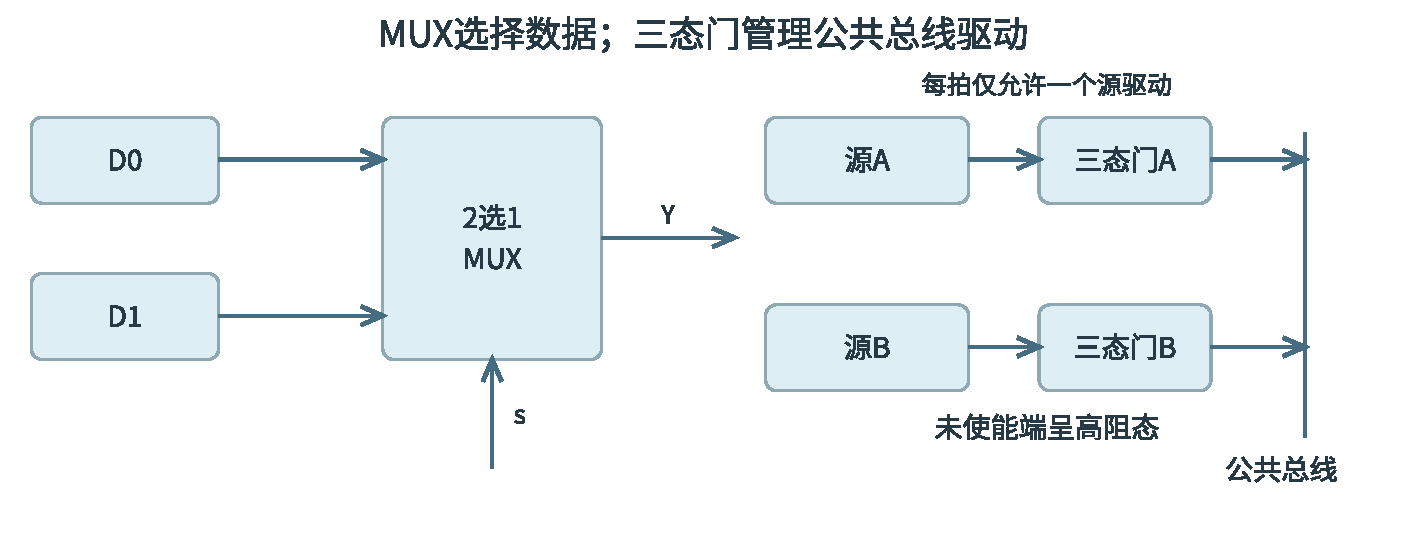
\includegraphics[width=\linewidth,height=108mm,keepaspectratio]{figures/CO02_mux_bus.pdf}
\caption{选择器选择数据源，三态门控制公共线驱动}
\end{figure}

\section{加减运算器与进位逻辑}\label{CO02-adder}

规定 \(C_i\) 为第 \(i\) 位输入进位，\(C_{i+1}\) 为输出进位：

\[S_i=A_i\oplus B_i\oplus C_i,\qquad G_i=A_iB_i,\quad P_i=A_i\oplus B_i,\]

\[C_{i+1}=G_i+P_iC_i.\]

例如 \(C_2=G_1+P_1G_0+P_1P_0C_0\)。串行进位逐级传播；先行进位用组合逻辑展开进位，增加电路复杂度以缩短关键路径。``并行输入各位''与``并行生成进位''是两项实现性质。

加减控制位 Sub 令第二输入为 \(B\oplus\mathrm{Sub}\)、最低进位 \(C_0=\mathrm{Sub}\)：

\[\mathrm{Sub}=0:\ A+B;\qquad \mathrm{Sub}=1:\ A+\overline B+1=A-B\pmod{2^n}.\]

ALU 按操作控制选择算术、与、或、异或等功能，移位器位置以具体通路为准。数据位宽与操作选择编码位宽分别确定。

\par\medskip\Needspace{4\baselineskip}\noindent\hypertarget{CO02-E04}{}\label{CO02-E04}\textbf{例 2-4}\par\nobreak\smallskip

某计算机字长为8位，CPU 中有一个8位加法器。已知无符号数 \(x=69,y=38\)，若在该加法器中计算 \(x-y\)，则加法器的两个输入端信息和输入的低位进位信息分别为（　）。

A. 0100 0101、0010 0110、0\\
B. 0100 0101、1101 1001、1\\
C. 0100 0101、1101 1010、0\\
D. 0100 0101、1101 1010、1

\section{运算标志与条件转移}\label{CO02-flags}

本章采用 CF=1表示减法借位的约定。设 \(n\) 位加减器最高输出进位为 \(C_n\)：

\[\mathrm{CF}=C_n\oplus\mathrm{Sub},\quad\mathrm{OF}=C_{n-1}\oplus C_n,\quad\mathrm{SF}=S_{n-1},\quad\mathrm{ZF}=[S=0].\]

CF 判断无符号溢出或借位；OF 判断补码有符号溢出。同号相加结果异号时加法溢出；异号相减结果与被减数异号时减法溢出。采用``无借位''进位约定的 ISA 应按其定义改判 CF。

\par\smallskip
{\fontsize{9.3}{12}\selectfont\setlength{\tabcolsep}{2.5pt}\setlength{\LTleft}{0pt}\setlength{\LTright}{0pt}
\begin{longtable}{@{}>{\raggedright\arraybackslash}p{\dimexpr0.16667\linewidth-2\tabcolsep\relax}>{\raggedright\arraybackslash}p{\dimexpr0.16667\linewidth-2\tabcolsep\relax}>{\raggedright\arraybackslash}p{\dimexpr0.16667\linewidth-2\tabcolsep\relax}>{\raggedright\arraybackslash}p{\dimexpr0.16667\linewidth-2\tabcolsep\relax}>{\raggedright\arraybackslash}p{\dimexpr0.16667\linewidth-2\tabcolsep\relax}>{\raggedright\arraybackslash}p{\dimexpr0.16667\linewidth-2\tabcolsep\relax}@{}}
\toprule
8位运算 & 低8位 & CF & OF & SF & ZF \\

\midrule\endfirsthead\toprule
8位运算 & 低8位 & CF & OF & SF & ZF \\

\midrule\endhead\bottomrule\endfoot
\texttt{7FH+01H} & \texttt{80H} & 0 & 1 & 1 & 0 \\

\texttt{FFH+01H} & \texttt{00H} & 1 & 0 & 0 & 1 \\

\texttt{80H-01H} & \texttt{7FH} & 0 & 1 & 0 & 0 \\

\texttt{00H-01H} & \texttt{FFH} & 1 & 0 & 1 & 0 \\

\end{longtable}}
\par\smallskip

计算 \(a-b\) 后的比较条件：

\par\smallskip
{\fontsize{9.3}{12}\selectfont\setlength{\tabcolsep}{2.5pt}\setlength{\LTleft}{0pt}\setlength{\LTright}{0pt}
\begin{longtable}{@{}>{\raggedright\arraybackslash}p{\dimexpr0.46508\linewidth-2\tabcolsep\relax}>{\raggedright\arraybackslash}p{\dimexpr0.53492\linewidth-2\tabcolsep\relax}@{}}
\toprule
条件 & 标志表达式 \\

\midrule\endfirsthead\toprule
条件 & 标志表达式 \\

\midrule\endhead\bottomrule\endfoot
相等 & ZF=1 \\

无符号 \(a<b\) & CF=1 \\

无符号 \(a>b\) & CF=0 且 ZF=0 \\

有符号 \(a<b\) & SF≠OF \\

有符号 \(a>b\) & SF=OF 且 ZF=0 \\

\end{longtable}}
\par\smallskip

\par\medskip\Needspace{4\baselineskip}\noindent\hypertarget{CO02-E05}{}\label{CO02-E05}\textbf{例 2-5}\par\nobreak\smallskip

假定有符号整数采用补码表示，若 int 型变量 x 和 y 的机器数分别是 FFFF FFDFH 和0000 0041H，则 x、y 的值及 x\ensuremath{-}y 的机器数分别是（　）。

A. x=\ensuremath{-}65，y=41，x\ensuremath{-}y 的机器数溢出\\
B. x=\ensuremath{-}33，y=65，x\ensuremath{-}y 的机器数为 FFFF FF9DH\\
C. x=\ensuremath{-}33，y=65，x\ensuremath{-}y 的机器数为 FFFF FF9EH\\
D. x=\ensuremath{-}65，y=41，x\ensuremath{-}y 的机器数为 FFFF FF96H

\par\medskip\Needspace{4\baselineskip}\noindent\hypertarget{CO02-E06}{}\label{CO02-E06}\textbf{例 2-6}\par\nobreak\smallskip

已知 x、y 为 int 类型，当 x=100、y=200时，执行``x减y''指令得到的溢出标志 OF 和借位标志 CF 分别为0、1。那么当 x=10、y=\ensuremath{-}20时，执行该指令得到的 OF 和 CF 分别是（　）。

A. OF=0，CF=0　 B. OF=0，CF=1　 C. OF=1，CF=0　 D. OF=1，CF=1

\section{无符号乘法与乘法器组织}\label{CO02-multiply}

两个 \(n\) 位数完整乘积最多需 \(2n\) 位。无符号顺序乘法初态 \(P=0\)，\(Y\) 装乘数，\(X\) 装被乘数。每轮：检查 \(Y_0\) \ensuremath{\to} 若为1则 \(P\leftarrow P+X\) 并保留进位 \ensuremath{\to} \((C,P,Y)\) 整体逻辑右移；共 \(n\) 轮。

\(X=1101,Y=1011\) 时：

\par\smallskip
{\fontsize{9.3}{12}\selectfont\setlength{\tabcolsep}{2.5pt}\setlength{\LTleft}{0pt}\setlength{\LTright}{0pt}
\begin{longtable}{@{}>{\raggedright\arraybackslash}p{\dimexpr0.28498\linewidth-2\tabcolsep\relax}>{\raggedright\arraybackslash}p{\dimexpr0.39386\linewidth-2\tabcolsep\relax}>{\raggedright\arraybackslash}p{\dimexpr0.32116\linewidth-2\tabcolsep\relax}@{}}
\toprule
轮次 & \(Y_0\)；加法后 \(C,P\) & 右移后 \(P,Y\) \\

\midrule\endfirsthead\toprule
轮次 & \(Y_0\)；加法后 \(C,P\) & 右移后 \(P,Y\) \\

\midrule\endhead\bottomrule\endfoot
初态 & --- & 0000,1011 \\

1 & 1；0,1101 & 0110,1101 \\

2 & 1；1,0011 & 1001,1110 \\

3 & 0；0,1001 & 0100,1111 \\

4 & 1；1,0001 & 1000,1111 \\

\end{longtable}}
\par\smallskip

结果 \texttt{10001111}=143。若只保存低 \(n\) 位，高 \(n\) 位非零表示无符号乘积溢出。

\par\smallskip
{\fontsize{9.3}{12}\selectfont\setlength{\tabcolsep}{2.5pt}\setlength{\LTleft}{0pt}\setlength{\LTright}{0pt}
\begin{longtable}{@{}>{\raggedright\arraybackslash}p{\dimexpr0.32881\linewidth-2\tabcolsep\relax}>{\raggedright\arraybackslash}p{\dimexpr0.67119\linewidth-2\tabcolsep\relax}@{}}
\toprule
乘法器组织 & 特征 \\

\midrule\endfirsthead\toprule
乘法器组织 & 特征 \\

\midrule\endhead\bottomrule\endfoot
顺序乘法器 & 复用加法器与移位器，跨多周期完成 \\

阵列乘法器 & 并行生成并压缩部分积，延迟由组合路径决定 \\

流水线乘法器 & 多级寄存器分隔组合路径，多组运算可重叠，提高吞吐率 \\

\end{longtable}}
\par\smallskip

常数乘法可在语义与位宽允许时化为移位加减，如 \(13x=(x\ll3)+(x\ll2)+x\)。

\subsection{Booth 补码一位乘法}\label{CO02-booth}

乘数后附 \(q_{-1}=0\)，每轮观察 \((Y_0,q_{-1})\)：00、11加0，01加 \(X\)，10减 \(X\)；随后 \((P,Y,q_{-1})\) 整体算术右移。符号位参加运算，跨寄存器边界传位。

\(X=1101=-3,Y=0110=6\)：

\par\smallskip
{\fontsize{9.3}{12}\selectfont\setlength{\tabcolsep}{2.5pt}\setlength{\LTleft}{0pt}\setlength{\LTright}{0pt}
\begin{longtable}{@{}>{\raggedright\arraybackslash}p{\dimexpr0.27018\linewidth-2\tabcolsep\relax}>{\raggedright\arraybackslash}p{\dimexpr0.33090\linewidth-2\tabcolsep\relax}>{\raggedright\arraybackslash}p{\dimexpr0.39892\linewidth-2\tabcolsep\relax}@{}}
\toprule
轮次 & 观察位与操作 & 右移后 \(P,Y,q_{-1}\) \\

\midrule\endfirsthead\toprule
轮次 & 观察位与操作 & 右移后 \(P,Y,q_{-1}\) \\

\midrule\endhead\bottomrule\endfoot
初态 & --- & 0000,0110,0 \\

1 & 00，加0 & 0000,0011,0 \\

2 & 10，减X & 0001,1001,1 \\

3 & 11，加0 & 0000,1100,1 \\

4 & 01，加X & 1110,1110,0 \\

\end{longtable}}
\par\smallskip

完整乘积 \texttt{11101110}=\ensuremath{-}18。保留低 \(n\) 位补码时，未溢出条件为完整积的高 \(n\) 位均为低半部符号位的扩展，即完整积最高 \(n+1\) 位全部相同。最小负数的取负及中间操作须配置足够保护位。

\section{除法、商溢出与余数校正}\label{CO02-division}

无符号双精度被除数以 \((R,Q)\) 保存，各 \(n\) 位，除数 \(Y\) 为 \(n\) 位。单精度被除数先零扩展。除数 \(Y>0\) 时，初始高半部 \(R\ge Y\) 意味着商至少为 \(2^n\)，产生商溢出。4位商中，255/15=17溢出，200/15=13余5可表示。

\par\smallskip
{\fontsize{9.3}{12}\selectfont\setlength{\tabcolsep}{2.5pt}\setlength{\LTleft}{0pt}\setlength{\LTright}{0pt}
\begin{longtable}{@{}>{\raggedright\arraybackslash}p{\dimexpr0.30902\linewidth-2\tabcolsep\relax}>{\raggedright\arraybackslash}p{\dimexpr0.69098\linewidth-2\tabcolsep\relax}@{}}
\toprule
算法 & 每轮更新与结束条件 \\

\midrule\endfirsthead\toprule
算法 & 每轮更新与结束条件 \\

\midrule\endhead\bottomrule\endfoot
恢复余数法 & 移入下一被除数位，试减除数；非负保留差、商位1；负则加回除数、商位0 \\

不恢复余数法 & 根据上一轮余数符号决定本轮减或加除数；按新余数生成商位；最终负余数须按规则校正 \\

\end{longtable}}
\par\smallskip

无符号最终结果必须满足 \(N=QY+R\) 且 \(0\le R<Y\)。试减的暂时负值需符号或借位状态支持。

\subsection{恢复余数法的寄存器轨迹}\label{CO02-restoring}

15/2 初态 \(R=0000,Q=1111,Y=0010\)，每轮先整体左移 \(RQ\)，再试减并记录商位，共4轮，得到 \(Q=0111,R=0001\)。

\begin{figure}[H]
\centering
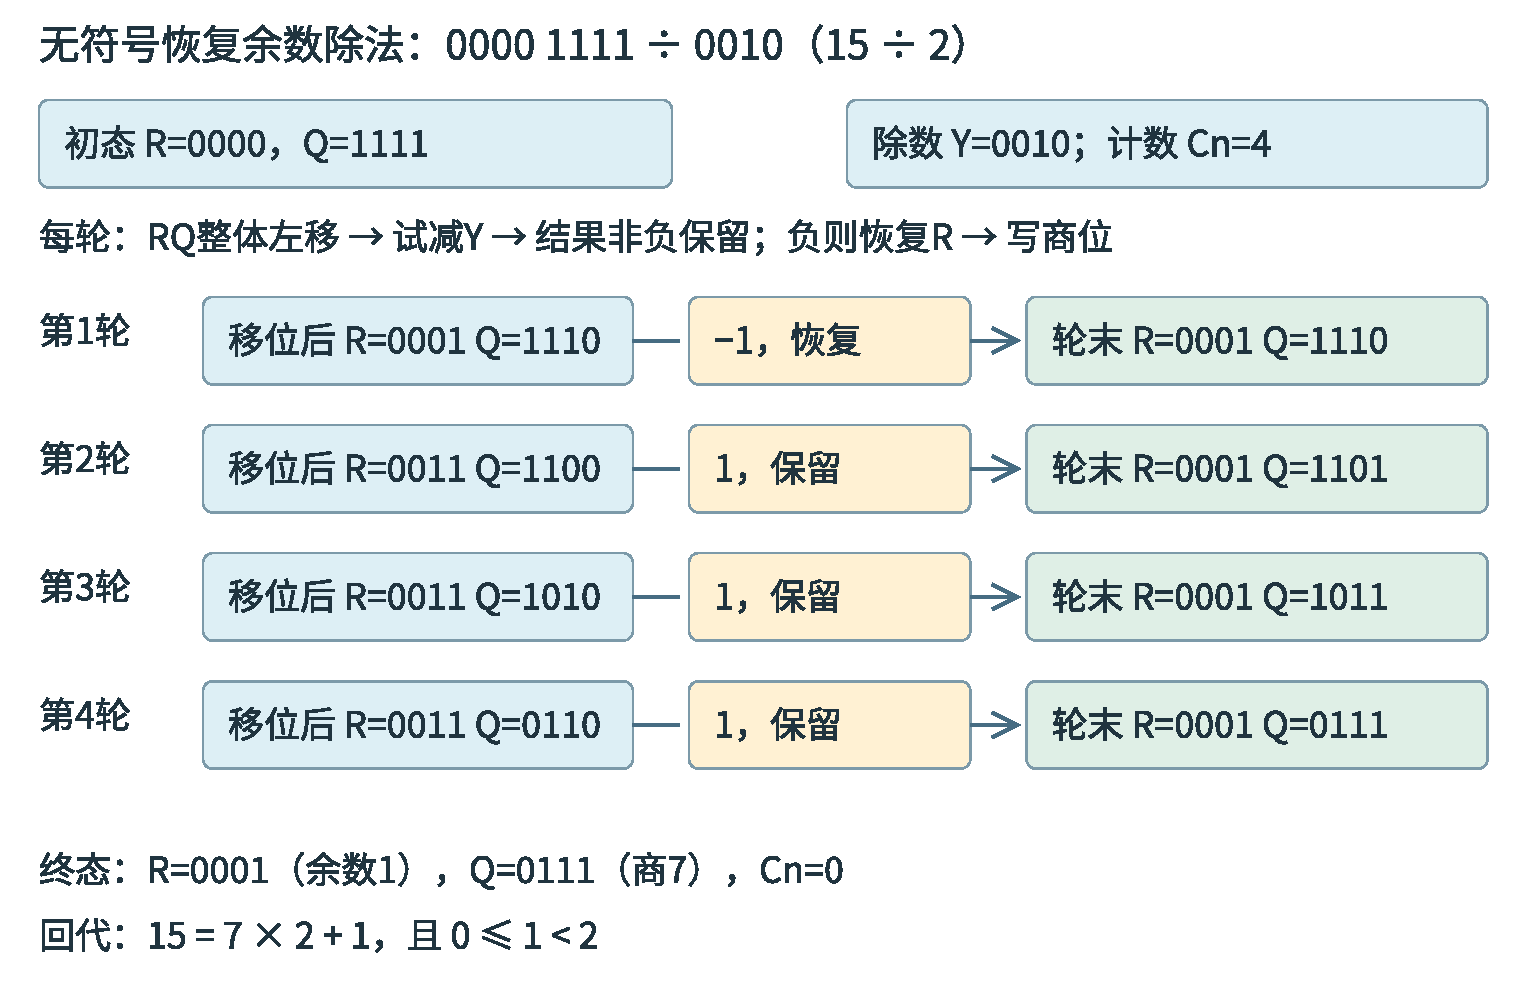
\includegraphics[width=\linewidth,height=108mm,keepaspectratio]{figures/CO02_restoring_division.pdf}
\caption{15除以2的试减、恢复和商位写入}
\end{figure}

不恢复余数法的7/3，取4位有符号 \(R\)、3位 \(Q\)：

\par\smallskip
{\fontsize{9.3}{12}\selectfont\setlength{\tabcolsep}{2.5pt}\setlength{\LTleft}{0pt}\setlength{\LTright}{0pt}
\begin{longtable}{@{}>{\raggedright\arraybackslash}p{\dimexpr0.19325\linewidth-2\tabcolsep\relax}>{\raggedright\arraybackslash}p{\dimexpr0.22701\linewidth-2\tabcolsep\relax}>{\raggedright\arraybackslash}p{\dimexpr0.19325\linewidth-2\tabcolsep\relax}>{\raggedright\arraybackslash}p{\dimexpr0.19325\linewidth-2\tabcolsep\relax}>{\raggedright\arraybackslash}p{\dimexpr0.19325\linewidth-2\tabcolsep\relax}@{}}
\toprule
轮次 & 整体左移后R & 本轮操作 & 操作后R & 记商后Q \\

\midrule\endfirsthead\toprule
轮次 & 整体左移后R & 本轮操作 & 操作后R & 记商后Q \\

\midrule\endhead\bottomrule\endfoot
初态 & --- & --- & 0 & 111 \\

1 & 1 & 减3 & −2 & 110 \\

2 & −3 & 加3 & 0 & 101 \\

3 & 1 & 减3 & −2 & 010 \\

\end{longtable}}
\par\smallskip

末轮 \(R<0\)，再加3校正为1；商2、余1。

\subsection{有符号除法与异常}\label{CO02-signed-division}

按向零截断约定，商符号由两操作数符号异或确定，非零余数与被除数同号，\(X=QY+R\)。例如\ensuremath{-}15/2的商\ensuremath{-}7、余\ensuremath{-}1；15/(\ensuremath{-}2)的商\ensuremath{-}7、余1。

课件4位补码\ensuremath{-}7/3：被除数符号扩展为 \(R=1111,Q=1001\)，\(Y=0011\)。本例负余数试加正除数；试加改变原负号时恢复，否则保留并生成商的绝对值位。

\par\smallskip
{\fontsize{9.3}{12}\selectfont\setlength{\tabcolsep}{2.5pt}\setlength{\LTleft}{0pt}\setlength{\LTright}{0pt}
\begin{longtable}{@{}>{\raggedright\arraybackslash}p{\dimexpr0.22735\linewidth-2\tabcolsep\relax}>{\raggedright\arraybackslash}p{\dimexpr0.25822\linewidth-2\tabcolsep\relax}>{\raggedright\arraybackslash}p{\dimexpr0.25621\linewidth-2\tabcolsep\relax}>{\raggedright\arraybackslash}p{\dimexpr0.25822\linewidth-2\tabcolsep\relax}@{}}
\toprule
轮次 & 左移后R、Q & 试加R & 轮末R、Q \\

\midrule\endfirsthead\toprule
轮次 & 左移后R、Q & 试加R & 轮末R、Q \\

\midrule\endhead\bottomrule\endfoot
1 & 1111、0010 & 0010，恢复 & 1111、0010 \\

2 & 1110、0100 & 0001，恢复 & 1110、0100 \\

3 & 1100、1000 & 1111，保留 & 1111、1001 \\

4 & 1111、0010 & 0010，恢复 & 1111、0010 \\

\end{longtable}}
\par\smallskip

最后商绝对值2，异号取补为1110=\ensuremath{-}2；余数1111=\ensuremath{-}1。整除时需单独正确接受试算零。也可在足够宽的内部表示中先求绝对值，完成无符号除法后恢复符号。

除数0须异常处理；\(-2^{n-1}/(-1)\) 超出 \(n\) 位补码商范围。固定轮数除法器按位宽迭代；提前退出须由题设明确给出。

\section{IEEE 754 字段与特殊值}\label{CO02-ieee}

设尾数字段整数值为 \(F\)、位数为 \(p\)、阶码为 \(E\)、偏置为 \(B\)，符号为 \(s\)。

\par\smallskip
{\fontsize{9.3}{12}\selectfont\setlength{\tabcolsep}{2.5pt}\setlength{\LTleft}{0pt}\setlength{\LTright}{0pt}
\begin{longtable}{@{}>{\raggedright\arraybackslash}p{\dimexpr0.35835\linewidth-2\tabcolsep\relax}>{\raggedright\arraybackslash}p{\dimexpr0.31649\linewidth-2\tabcolsep\relax}>{\raggedright\arraybackslash}p{\dimexpr0.32516\linewidth-2\tabcolsep\relax}@{}}
\toprule
参数 & binary32 & binary64 \\

\midrule\endfirsthead\toprule
参数 & binary32 & binary64 \\

\midrule\endhead\bottomrule\endfoot
符号／阶码／尾数字段位数 & 1／8／23 & 1／11／52 \\

偏置 \(B\) & 127 & 1023 \\

规格化有效精度 & 24位 & 53位 \\

规格化真阶码 & −126～127 & −1022～1023 \\

最小正规格化数 & \(2^{-126}\) & \(2^{-1022}\) \\

最小正次正规数 & \(2^{-149}\) & \(2^{-1074}\) \\

最大有限正数 & \((2-2^{-23})2^{127}\) & \((2-2^{-52})2^{1023}\) \\

\end{longtable}}
\par\smallskip

\par\smallskip
{\fontsize{9.3}{12}\selectfont\setlength{\tabcolsep}{2.5pt}\setlength{\LTleft}{0pt}\setlength{\LTright}{0pt}
\begin{longtable}{@{}>{\raggedright\arraybackslash}p{\dimexpr0.34979\linewidth-2\tabcolsep\relax}>{\raggedright\arraybackslash}p{\dimexpr0.65021\linewidth-2\tabcolsep\relax}@{}}
\toprule
字段条件 & 数值／含义 \\

\midrule\endfirsthead\toprule
字段条件 & 数值／含义 \\

\midrule\endhead\bottomrule\endfoot
\(E=0,F=0\) & 正零或负零，由 \(s\) 区分 \\

\(E=0,F\ne0\) & 次正规数（非规格化数），\((-1)^s(F/2^p)2^{1-B}\)，隐含前导0 \\

\(E\) 既非全0也非全1 & 规格化数，\((-1)^s(1+F/2^p)2^{E-B}\)，隐含前导1 \\

\(E\) 全1，\(F=0\) & 正无穷或负无穷 \\

\(E\) 全1，\(F\ne0\) & NaN \\

\end{longtable}}
\par\smallskip

\begin{figure}[H]
\centering
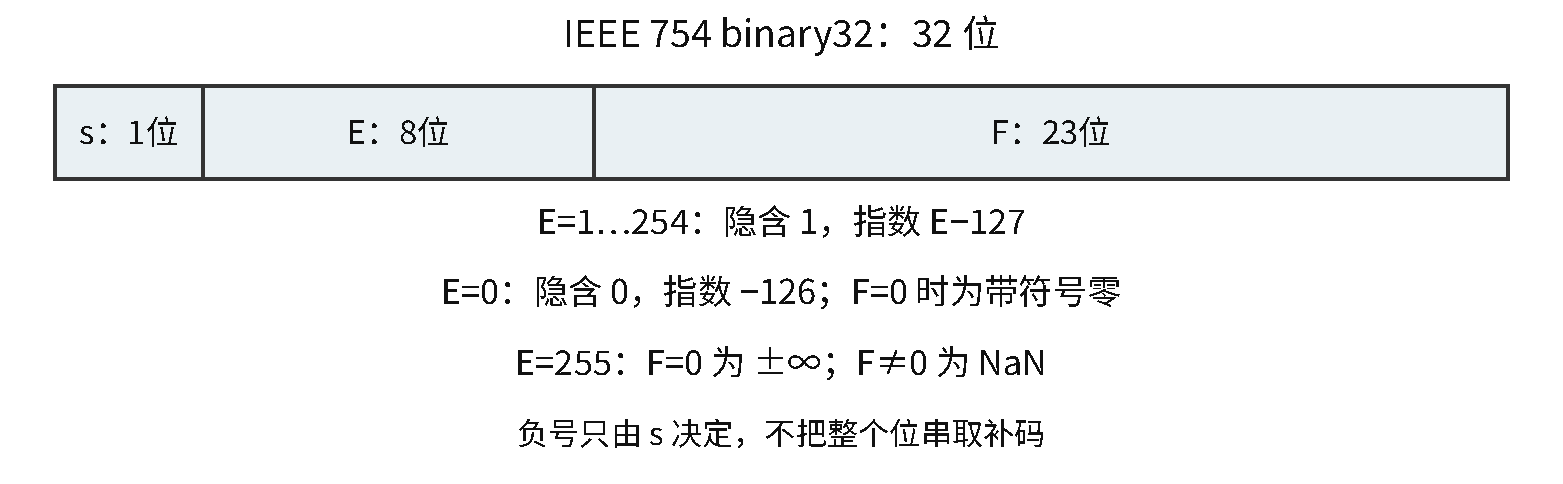
\includegraphics[width=\linewidth,height=108mm,keepaspectratio]{figures/CO_F01_ieee754.pdf}
\caption{单精度字段与指数编码}
\end{figure}

binary32位串 \texttt{00000001H} 为 \(2^{-149}\)，\texttt{00800000H} 为 \(2^{-126}\)。编码前先规格化绝对值，最后独立写符号位；负浮点数按符号、指数、尾数解读。比较有限同号负数时，绝对值较大者数值较小。

\par\medskip\Needspace{4\baselineskip}\noindent\hypertarget{CO02-E07}{}\label{CO02-E07}\textbf{例 2-7}\par\nobreak\smallskip

\ensuremath{-}0.4375的 IEEE 754 单精度浮点数表示为（　）。

A. BEE0 0000H　 B. BF60 0000H　 C. BF70 0000H　 D. C0E0 0000H

\par\medskip\Needspace{4\baselineskip}\noindent\hypertarget{CO02-E08}{}\label{CO02-E08}\textbf{例 2-8}\par\nobreak\smallskip

float 型数据常用 IEEE 754 单精度浮点格式表示。假设两个 float 型变量 x 和 y 分别存放在32位寄存器 f1 和 f2 中，若 \texttt{(\allowbreak{}f1)\allowbreak{}=\allowbreak{}CC90 0000H}、\texttt{(\allowbreak{}f2)\allowbreak{}=\allowbreak{}B0C0 0000H}，则 x 和 y 之间的关系为（　）。

A. x\textless y且符号相同　 B. x\textless y且符号不同　 C. x\textgreater y且符号相同　 D. x\textgreater y且符号不同

\section{浮点加减与舍入}\label{CO02-float-operation}

顺序为：对阶 \ensuremath{\to} 尾数加减 \ensuremath{\to} 规格化 \ensuremath{\to} 舍入 \ensuremath{\to} 检查规格化与阶码范围。

\par\smallskip
{\fontsize{9.3}{12}\selectfont\setlength{\tabcolsep}{2.5pt}\setlength{\LTleft}{0pt}\setlength{\LTright}{0pt}
\begin{longtable}{@{}>{\raggedright\arraybackslash}p{\dimexpr0.26748\linewidth-2\tabcolsep\relax}>{\raggedright\arraybackslash}p{\dimexpr0.73252\linewidth-2\tabcolsep\relax}@{}}
\toprule
步骤 & 规则与边界 \\

\midrule\endfirsthead\toprule
步骤 & 规则与边界 \\

\midrule\endhead\bottomrule\endfoot
对阶 & 小阶向大阶对齐，小阶尾数右移；最终阶码为原合法大阶，可能损失低位 \\

右规 & 尾数出现 \(10.xxx_2\) 时右移1位、阶码加1，可能上溢 \\

左规 & 抵消后左移尾数、阶码减少，可能触及次正规区或下溢边界；精确零单独处理 \\

舍入 & 可能使尾数进位，再右规并检查上溢 \\

渐进下溢 & 指数过小时可能形成次正规数，接近0后才舍入为零 \\

\end{longtable}}
\par\smallskip

最近偶数舍入：被舍部分小于半个间隔取低端，大于半个间隔取高端，恰好居中取保留有效数最低位为0的候选。保护位 G、舍入位 R、粘滞位 S 保留舍入依据，S 为更低被舍位的逻辑或；最近偶数下，\(G=1\) 且 \((R\lor S\lor\mathrm{LSB})=1\) 时向保留部分进1。

\par\medskip\Needspace{4\baselineskip}\noindent\hypertarget{CO02-E09}{}\label{CO02-E09}\textbf{例 2-9}\par\nobreak\smallskip

下列有关浮点数加减运算的叙述中，正确的是（　）。

I. 对阶操作不会引起阶码上溢或下溢\\
II. 右规和尾数舍入都可能引起阶码上溢\\
III. 左规时可能引起阶码下溢\\
IV. 尾数溢出时，结果不一定溢出

A. 仅 II、III　 B. 仅 I、II、IV　 C. 仅 I、III、IV　 D. I、II、III、IV

浮点加法可能不满足结合律。binary32取 \(a=2^{25},b=-2^{25},c=1\)，则 \((a+b)+c=1\)，而 \(b+c\) 先舍入回 \(b\)，得到 \(a+(b+c)=0\)。

\subsection{浮点精度与数值范围}\label{CO02-precision}

binary32 在 \([2^e,2^{e+1})\) 中的相邻正规格化数间隔为 \(2^{e-23}\)。所有 \([-2^{24},2^{24}]\) 内整数可精确表示，界外部分整数仍可精确表示；在 \([2^{24},2^{25})\) 中间隔2，在 \([2^{25},2^{26})\) 中间隔4。

\par\smallskip
{\fontsize{9.3}{12}\selectfont\setlength{\tabcolsep}{2.5pt}\setlength{\LTleft}{0pt}\setlength{\LTright}{0pt}
\begin{longtable}{@{}>{\raggedright\arraybackslash}p{\dimexpr0.43323\linewidth-2\tabcolsep\relax}>{\raggedright\arraybackslash}p{\dimexpr0.56677\linewidth-2\tabcolsep\relax}@{}}
\toprule
精确数学结果 & binary32 最近偶数结果 \\

\midrule\endfirsthead\toprule
精确数学结果 & binary32 最近偶数结果 \\

\midrule\endhead\bottomrule\endfoot
\(2^{24}+0.5\) & 16777216 \\

\(2^{24}+1\) & 16777216 \\

\(2^{24}+1.5\) & 16777218 \\

\((2^{24}+2)+1\) & 16777220 \\

\end{longtable}}
\par\smallskip

精确性由有效位与舍入决定，有限范围由指数和尾数上界共同决定。32位补码在其范围内表示连续整数；binary32的数值范围较大、有效精度为24位。

\par\medskip\Needspace{4\baselineskip}\noindent\hypertarget{CO02-E10}{}\label{CO02-E10}\textbf{例 2-10}\par\nobreak\smallskip

已知 \(f(n)=\sum_{i=0}^{n}2^i=2^{n+1}-1=\underbrace{11\cdots1}_{n+1\text{位}}{}_2\)，计算 \(f(n)\) 的C语言函数f1如下。

\par\smallskip\noindent\begin{minipage}{\linewidth}
\begin{codeblock}[language={C}]
int f1(unsigned n) {
    int sum = 1, power = 1;
    for (unsigned i = 0; i <= n - 1; i++) {
        power *= 2;
        sum += power;
    }
    return sum;
}
\end{codeblock}
\end{minipage}\par\smallskip

将f1中的int都改为float，可得到计算 \(f(n)\) 的另一个函数f2。假设unsigned和int型数据都占32位，float采用IEEE 754单精度标准。请回答下列问题。

（1）当n=0时，f1会出现死循环，为什么？若将f1中的变量i和n都定义为int型，则f1是否还会出现死循环？为什么？

（2）f1(23)和f2(23)的返回值是否相等？机器数各是什么（用十六进制表示）？

（3）f1(24)和f2(24)的返回值分别为33 554 431和33 554 432.0，为什么不相等？

（4）\(f(31)=2^{32}-1\)，而f1(31)的返回值却为\ensuremath{-}1，为什么？若使f1(n)的返回值与f(n)相等，则最大的n是多少？

（5）f2(127)的机器数为7F80 0000H，对应的值是什么？若使f2(n)的结果不溢出，则最大的n是多少？若使f2(n)的结果精确（无舍入），则最大的n是多少？

32位 int 转 binary64 可精确，转 binary32 可能丢低位。binary32有限值扩为 binary64 可精确保留，已经丢失的信息无法恢复。浮点转整数向零截断且须检查目标范围；NaN 与任何值含自身的相等比较为假。

\section{字节序、边界对齐与数组地址}\label{CO02-storage}

\par\smallskip
{\fontsize{9.3}{12}\selectfont\setlength{\tabcolsep}{2.5pt}\setlength{\LTleft}{0pt}\setlength{\LTright}{0pt}
\begin{longtable}{@{}>{\raggedright\arraybackslash}p{\dimexpr0.30204\linewidth-2\tabcolsep\relax}>{\raggedright\arraybackslash}p{\dimexpr0.69796\linewidth-2\tabcolsep\relax}@{}}
\toprule
存放规则 & 最低地址保存的字节 \\

\midrule\endfirsthead\toprule
存放规则 & 最低地址保存的字节 \\

\midrule\endhead\bottomrule\endfoot
大端 & 最高有效字节；\texttt{12345678H} 依次12、34、56、78 \\

小端 & 最低有效字节；\texttt{12345678H} 依次78、56、34、12 \\

\end{longtable}}
\par\smallskip

字节序只改变一个多字节对象内部各字节的位置，字节内位序、数组元素先后次序保持各自规定。\ensuremath{-}6的16位补码 \texttt{FFFAH} 按小端存为FA、FF。

自然对齐模型下，2 B对象起点为2的倍数，4 B对象起点为4的倍数。成员前填充满足各成员对齐，结构末尾填充满足相邻数组元素对齐，具体规则由题设或 ABI 给出。

成员偏移可按 \(\lceil d/a\rceil a\) 对齐，其中 \(d\) 为前一成员结束后的偏移，\(a\) 为当前成员对齐要求。结构总长按结构对齐要求取整。

\par\medskip\Needspace{4\baselineskip}\noindent\hypertarget{CO02-E11}{}\label{CO02-E11}\textbf{例 2-11}\par\nobreak\smallskip

某计算机存储器按字节编址，采用小端方式存放数据。假定编译器规定 int 型和 short 型长度分别为32位和16位，并且数据按边界对齐存储。某 C 语言程序段如下：

\par\smallskip\noindent\begin{minipage}{\linewidth}
\begin{codeblock}[language={C}]
struct {
    int a;
    char b;
    short c;
} record;
record.a = 273;
\end{codeblock}
\end{minipage}\par\smallskip

若 record 变量的首地址为0xC008，则地址0xC008中的内容及 record.c 的地址分别为（　）。

A. 0x00，0xC00D　 B. 0x00，0xC00E\\
C. 0x11，0xC00D　 D. 0x11，0xC00E

\begin{figure}[H]
\centering
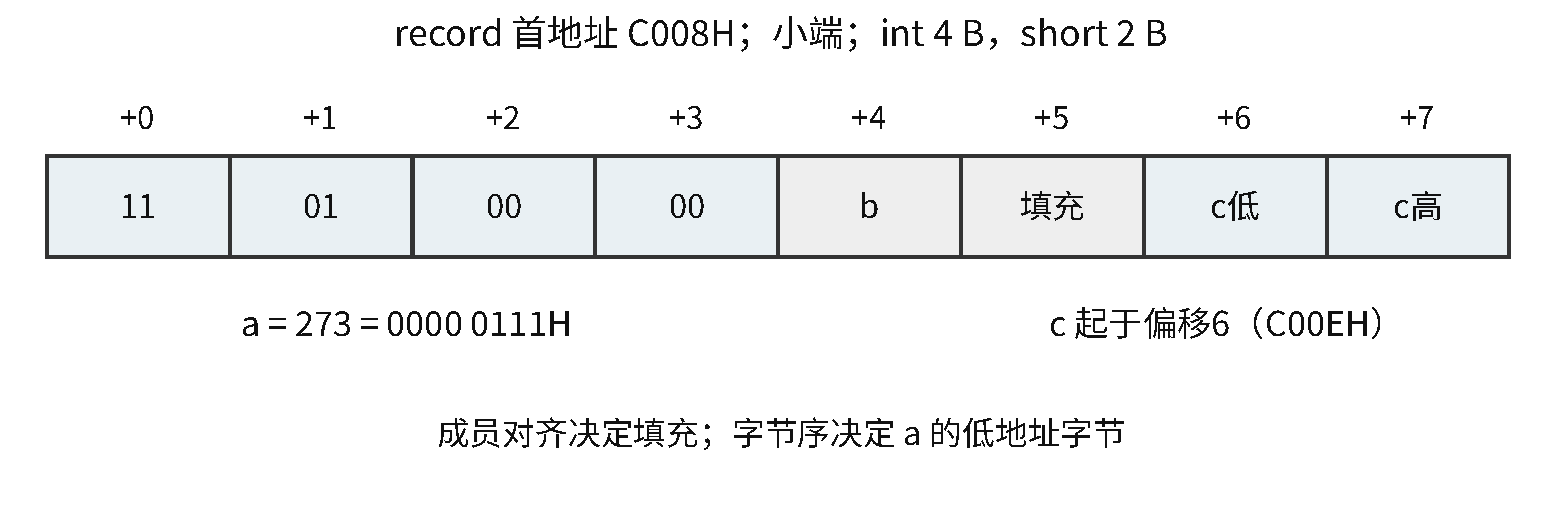
\includegraphics[width=\linewidth,height=108mm,keepaspectratio]{figures/CO_F05_struct_layout.pdf}
\caption{结构体成员与填充位置}
\end{figure}

按字节编址、元素宽 \(w\) B、行优先二维数组列数 \(C\)：

\[\operatorname{addr}(a[i][j])=\operatorname{base}(a)+(iC+j)w.\]

\texttt{struct \{ int id;\allowbreak{} char name[\allowbreak{}10]\allowbreak{};\allowbreak{} int salary;\allowbreak{} \}} 在 int为4 B且自然对齐时，id偏移0，name偏移4，salary偏移16，结构长20 B。数组首址 A0B0H，第二元素 id=\texttt{12345678H} 时，小端字节56H位于 A0C5H。

机器字长、存储字长与指令字长分别确定。按字节编址的32位整数占4个地址，按32位字编址则占1个地址；容量与跨界访问均先统一地址单位。
